\subsection{Dynamic Model (without Propeller)}
We have the dynamic model of BLDC motor using moment balance:
\begin{align*}
    J_m \dot \omega_m &= T_e - b_f \omega_m - M_f\\
    \text{where, } \qquad &\\
    J_m &- \text{Moment of inertia of the motor}\\
    b_f &- \text{lumped parameter for viscous friction}\\
    M_f &- \text{lumped parameter for coulomb friction}
\end{align*}
\itbf{Friction:}
\begin{enumerate}
    \item Viscous friction: $-b_f \omega$.
    \item Columb friction: $-M_{f} \sign(\omega) = -M_{f} \qquad [\because$ the motor turns in only one direction $]$.
\end{enumerate}

\medskip

From the speed-torque characteristics of the BLDC motor:
\begin{align*}
    T_e &= K_T I = K_T \frac{(V_s - E)}{R} = \frac{K_T}{R} (V_s - K_v \omega_m)  & [\because K_v = K_T = k \psi]\\
    \text{Let, }\qquad \qquad &\\
    K_r &= \frac{K_T}{R}
\end{align*}
From the definition of Input to ESC:
\begin{align*}
    V_s &= u V_{in}\\
    \therefore T_e &= u K_r V_{in} - K_r K_v \omega_m
\end{align*}

Substituting:
\begin{align*}
    &J_m \dot \omega_m = u K_r V_{in}  - K_rK_v \omega_m  - b_f \omega_m - M_f
\end{align*}
\begin{equation}
    \boxed{
    J_m \dot \omega_m + (K_r K_v  + b_f) \omega_m + M_f = u K_r V_{in}
    }
    \label{eqn:no_prop}
\end{equation}

\subsection{BLDC Motor with Propeller}
Adding propeller moment of inertia and the moment due to propeller drag into the BLDC motor model.
\begin{align*}
    (J_m + J_p) \dot \omega + (K_rK_v + b_f) \omega + M_f &= u K_r V_{in} - C_D \omega^2
\end{align*}
Where, $C_D$ is the aerodynamic drag. Let, $J_m + J_p = J$
\begin{equation}
    \boxed{
    J\dot \omega + (K_rK_v + b_f) \omega + C_D \omega^2 + M_f = u K_r V_{in}
    }
    \label{eqn:prop}
\end{equation}


%    \text{Substituting, } \quad K_r u &= (K_r K_v  + b_f) u_\omega + \frac{M_f}{\hat V_{in}}\\
%   J\dot \omega + (K_rK_v + b_f) \omega + C_D \omega^2 + M_f &= V_{in} \left((K_r K_v  + b_f) u_\omega + \frac{M_f}{\hat V_{in}} \right)\\



% \begin{align*}
%     \text{Using normalized no-load angular velocity input:} &\\
%     J_m \dot \omega_m + (K_r K_v  + b_f) \omega_m + M_f &= \left(\left(\frac{K_r K_v  + b_f}{K_r} \right) u_{\omega} + \frac{M_f}{K_r \hat V_{in}} \right) K_r V_{in}\\
%     &= V_{in}(K_r K_v  + b_f)u_{\omega} + M_f \frac{V_{in}}{\hat V_{in}}
% \end{align*}

% We get the linearised model using small perturbtation:
% \begin{align*}
%     J_m \delta \dot \omega_m + (K_rK_v + b_f) \delta  \omega_m  &= \delta u_{\omega}V_{in}(K_r K_v  + b_f) \\
%     \frac{\delta \omega_m (s)}{\delta u (s)} &= \frac{V_{in}(K_r K_v  + b_f)}{J_m s + (K_r K_v + b_f)} = \frac{V_{in}}{\frac{J_m}{(K_r K_v + b_f)} s + 1} = \frac{K_m}{\tau_m s + 1}\\
%     \text{where, }\qquad &\\
%     K_m &= V_{in}\\
%     \tau_m &= \frac{J_m}{(K_rK_v + b_f)}
% \end{align*}

% \begin{minipage}{0.49\textwidth}
% Writing interms of $\delta u_p$:
% \begin{align*}
%    \delta u_\omega &= g'_w(u_p) \delta u_p\\
%    \implies \frac{\delta \omega_m (s)}{\delta u_{p} (s)} &= \frac{K g'_w(u_p)}{\tau s + 1}
% \end{align*}
% This explains the static gain variation observed in the system identification.
% \end{minipage}
% \begin{minipage}{0.49\textwidth}
%  \begin{figure}[H]
%     \centering
%     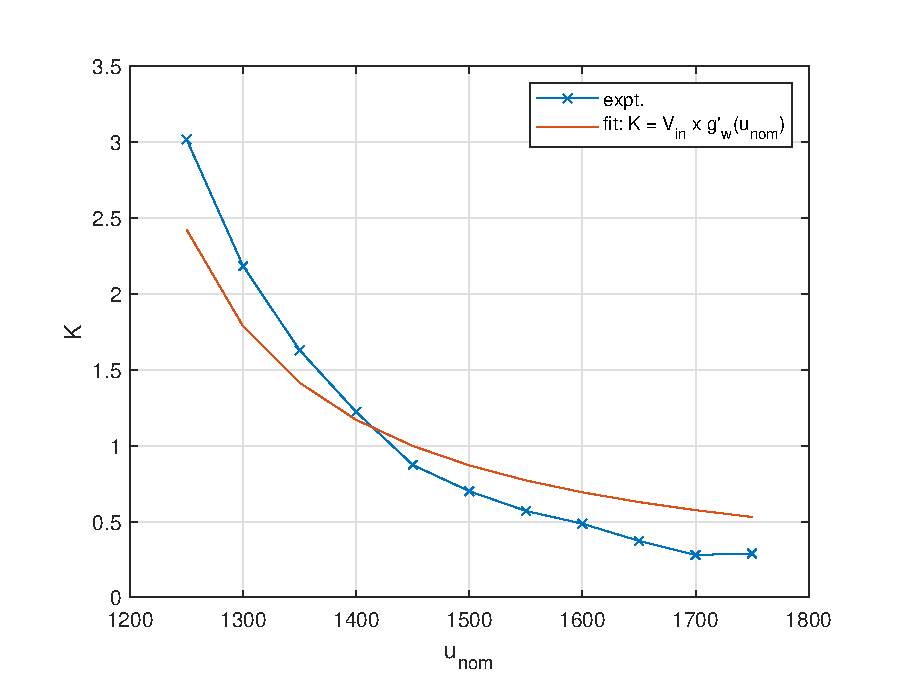
\includegraphics[width = \textwidth]{./figs/norm_omega/K_fit.eps}
%     \caption{Static gain variation with nominal input ($u_p$) with input perturbtation $\delta u_p = 100 \mu s$}
% \end{figure}
% \end{minipage}
% %===============================================================================
%\subsection{Parametric Identification model for BLDC motor dyanmcis}
%\subsubsection{Continuous Parametric Model}
%\begin{align*}
%    J_m \dot \omega &= -(K_rK_v + b_f) \omega_m - M_f + u K_r V_{in}\\
%   %===
%    \implies \dot \omega &= -\frac{(K_rK_v + b_f)}{J_m} \omega_m - \frac{M_f}{J_m} + u \frac{K_r V_{in}}{J_m}
%\end{align*}
%
%Hence, we have the continuous parametric model:
%$$ \dot \omega =
%    \underbrace{\begin{bmatrix}
%               - \omega  & -1
%\end{bmatrix}}_{\Phi^T(\omega)}
%\underbrace{\begin{bmatrix}
%    \frac{(K_rK_v + b_f)}{J_m}  \\
%    \frac{M_f}{J_m}
%\end{bmatrix} }_{\pmb \theta}
%    +\frac{K_r V_{in}}{J_m}u $$
%
%Let,
%\begin{align*}
%    a_1 &= \frac{(K_rK_v + b_f)}{J_m} \qquad
%    a_2 =   \frac{M_f}{J_m}\\
%    \\
%    \pmb \theta &= \begin{bmatrix}a_1 & a_2 \end{bmatrix}^T \qquad
%    b =  \frac{K_r V_{in}}{J_m}
%\end{align*}
%
%$$\therefore \dot \omega = \Phi^T(\omega) \pmb \theta + b u$$
%
%\subsubsection{Descritezed Parametric Model}
%Descritizing the above model using euler-method $\left(\dot \omega = \frac{\omega[k] - \omega[k-1]}{h}\right)$, with $h$ as the sampling interval:
%
%\begin{align*}
%    \frac{\omega[k] - \omega[k-1]}{h} &=
%    \begin{bmatrix}  - \omega[k-1]  &  -1 \end{bmatrix}
%    \begin{bmatrix}
%        a_1 \\ a_2
%    \end{bmatrix}
%    + bu[k-1]\\
%    %===
%    \omega[k] &= h \begin{bmatrix} - \omega[k-1]  & -1 \end{bmatrix}
%    \begin{bmatrix}
%        a_1 - \frac{1}{h} \\
%        a_2 \\
%    \end{bmatrix}
%    + b  h u[k-1]\\
%    %===
%    &= h \begin{bmatrix} -\omega[k-1] & -1 & u[k] \end{bmatrix}
%    \begin{bmatrix}
%        a_1 - \frac{1}{h} \\
%        a_2 \\
%        b
%    \end{bmatrix}
%\end{align*}
%
%Let,
%\begin{align*}
%    \pmb \theta_h = h
%    \begin{bmatrix}
%        a_1 - \frac{1}{h} \\
%        a_2 \\
%        b
%    \end{bmatrix} =
%    h
%    \begin{bmatrix}
%        \frac{(K_rK_v + b_f)}{J_m} - \frac{1}{h}  \\
%        \frac{M_f}{J_m}\\
%        \frac{K_r V_{in}}{J_m}
%    \end{bmatrix}
%    \qquad \text{and} \qquad
%    \Phi(\omega[k-1], u[k])^T &=  \begin{bmatrix}  -\omega[k-1] & -1 & u[k-1] \end{bmatrix}
%\end{align*}
%
%hence, we have the parametric model in least-squares form:
%\begin{align*}
%    \omega[k] &= \Phi(\omega[k-1], u[k-1])^T \pmb \theta_h
%\end{align*}
%
